\documentclass[11pt,a4paper]{article}

\usepackage[utf8]{inputenc}
\usepackage{lmodern}  % Use Latin Modern fonts instead of cm-super
\usepackage[T1]{fontenc}
\usepackage{amsmath,amssymb,amsfonts}
\usepackage{booktabs}
\usepackage{array}
\usepackage{colortbl}  % For \rowcolor in tables
\usepackage{xcolor}
\usepackage{tikz}
\usetikzlibrary{arrows.meta,positioning,shapes.geometric}
\usepackage{graphicx}
\usepackage{geometry}
\geometry{margin=2.5cm}
\usepackage{listings}
\usepackage{xcolor}

\definecolor{codegreen}{rgb}{0,0.6,0}
\definecolor{codegray}{rgb}{0.5,0.5,0.5}
\definecolor{codepurple}{rgb}{0.58,0,0.82}
\definecolor{backcolour}{rgb}{0.95,0.95,0.92}

\lstdefinestyle{mystyle}{
    backgroundcolor=\color{backcolour},
    commentstyle=\color{codegreen},
    keywordstyle=\color{magenta},
    numberstyle=\tiny\color{codegray},
    stringstyle=\color{codepurple},
    basicstyle=\ttfamily\footnotesize,
    breakatwhitespace=false,
    breaklines=true,
    captionpos=b,
    keepspaces=true,
    numbers=left,
    numbersep=5pt,
    showspaces=false,
    showstringspaces=false,
    showtabs=false,
    tabsize=2
}

\lstset{style=mystyle}

\usepackage[hidelinks,pdfencoding=auto]{hyperref}

\title{Biologically-Constrained Parameter Reduction\\for 5-Species Biofilm Model}
\author{Keisuke Nishioka}
\date{February 2026}

\begin{document}

\maketitle

\begin{abstract}
This document describes the Proposed Method, a parameter reduction technique for Bayesian estimation of the 5-species biofilm interaction model. By incorporating biological knowledge from experimentally determined interaction networks, the algorithm reduces the parameter space from 20 to 15 free parameters, improving estimation efficiency and biological interpretability.

\vspace{0.5cm}
\noindent\textbf{Keywords:} Bayesian Estimation, Biofilm, Parameter Reduction, TMCMC, Biological Constraints, Multi-species Interaction, Inverse Problem, Peri-implantitis, Uncertainty Quantification
\end{abstract}

\tableofcontents
\newpage

%==============================================================================
\section{Introduction}
%==============================================================================

Understanding the dynamics of multi-species biofilms is crucial for the prevention and treatment of oral diseases. Heine et al. \cite{Heine2025PeriImplant} investigated the interactions of five major oral bacterial species associated with peri-implantitis. Based on these experimental findings and the extended Hamilton principle proposed by Junker and Balzani \cite{JunkerBalzani2021ExtendedHamilton}, Klempt et al. \cite{Klempt2025ContinuumBiofilm} developed a continuum model for multi-species biofilms with a novel interaction scheme. Furthermore, Fritsch et al. \cite{Fritsch2025BayesianMicrofilms} discussed Bayesian updating methods for bacterial microfilms under hybrid uncertainties using a novel surrogate model.

The 5-species biofilm model describes the dynamics of bacterial populations through an interaction matrix $\mathbf{A}$ and decay vector $\mathbf{b}$. However, the standard parameter estimation approach estimates all 20 parameters freely, which can lead to:

\begin{itemize}
    \item Poor identifiability due to limited experimental data
    \item Biologically implausible parameter estimates
    \item Computational inefficiency from exploring unnecessary parameter space
\end{itemize}

The Proposed Method addresses these issues by constraining certain interaction parameters to zero based on experimental evidence of absent species interactions.

%==============================================================================
\section{Biological Basis}
%==============================================================================

\subsection{Species in the Model}

The model includes five bacterial species commonly found in oral biofilms:

\begin{table}[h]
\centering
\begin{tabular}{clll}
\toprule
\textbf{ID} & \textbf{Species} & \textbf{Abbrev.} & \textbf{Role} \\
\midrule
0 & \textit{Streptococcus oralis} & S.o & Early colonizer \\
1 & \textit{Actinomyces naeslundii} & A.n & Early colonizer \\
2 & \textit{Veillonella} spp. & Vei & Metabolic bridge \\
3 & \textit{Fusobacterium nucleatum} & F.n & Bridge organism \\
4 & \textit{Porphyromonas gingivalis} & P.g & Late colonizer (pathogen) \\
\bottomrule
\end{tabular}
\caption{Species included in the 5-species biofilm model.}
\label{tab:species}
\end{table}

\subsection{Interaction Network (Figure 4C)}

Based on experimental observations \cite{Heine2025PeriImplant}, the following interaction network was established:

\begin{figure}[h]
\centering
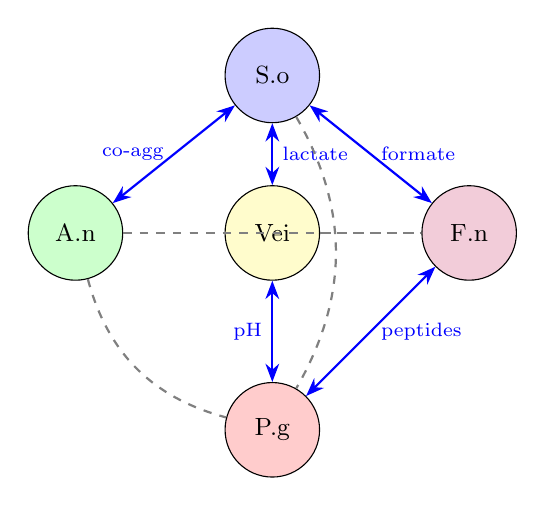
\begin{tikzpicture}[
    node distance=2.5cm,
    species/.style={circle, draw, minimum size=1.2cm, font=\small},
    edge/.style={<->, thick, >=Stealth},
    noedge/.style={dashed, gray, thick}
]
    % Nodes
    \node[species, fill=blue!20] (so) at (0, 3) {S.o};
    \node[species, fill=green!20] (an) at (-2.5, 1) {A.n};
    \node[species, fill=yellow!20] (vei) at (0, 1) {Vei};
    \node[species, fill=purple!20] (fn) at (2.5, 1) {F.n};
    \node[species, fill=red!20] (pg) at (0, -1.5) {P.g};

    % Active edges (solid)
    \draw[edge, blue] (so) -- (an) node[midway, left, font=\scriptsize] {co-agg};
    \draw[edge, blue] (so) -- (vei) node[midway, right, font=\scriptsize] {lactate};
    \draw[edge, blue] (so) -- (fn) node[midway, right, font=\scriptsize] {formate};
    \draw[edge, blue] (vei) -- (pg) node[midway, left, font=\scriptsize] {pH};
    \draw[edge, blue] (fn) -- (pg) node[midway, right, font=\scriptsize] {peptides};

    % Locked edges (dashed, crossed out)
    \draw[noedge] (an) -- (vei);
    \draw[noedge] (an) -- (fn);
    \draw[noedge] (vei) -- (fn);
    \draw[noedge] (so) to[bend left=30] (pg);
    \draw[noedge] (an) to[bend right=30] (pg);

\end{tikzpicture}
\caption{Species interaction network derived from Figure 4C. Solid blue arrows indicate active interactions (estimated parameters). Dashed gray lines indicate absent interactions (locked to zero).}
\label{fig:network}
\end{figure}

\subsection{Active Interactions}

The following species pairs have direct biological interactions:

\begin{table}[h]
\centering
\begin{tabular}{lll}
\toprule
\textbf{Species Pair} & \textbf{Mechanism} & \textbf{Type} \\
\midrule
S. oralis $\leftrightarrow$ A. naeslundii & Co-aggregation & Bidirectional \\
S. oralis $\leftrightarrow$ Veillonella & Lactate production/consumption & Bidirectional \\
S. oralis $\leftrightarrow$ F. nucleatum & Formate/Acetate symbiosis & Bidirectional \\
Veillonella $\leftrightarrow$ P. gingivalis & pH rise support & Positive only \\
F. nucleatum $\leftrightarrow$ P. gingivalis & Co-aggregation, peptides & Bidirectional \\
\bottomrule
\end{tabular}
\caption{Active species interactions with biological mechanisms.}
\label{tab:active}
\end{table}

\subsection{Absent Interactions (Locked)}

The following species pairs have no direct interaction according to experimental evidence (Figure 4C). These are locked to zero ($\theta_k = 0$) in the Proposed Method:

\begin{table}[h]
\centering
\begin{tabular}{cllll}
\toprule
\textbf{Index} & \textbf{Param} & \textbf{Species Pair} & \textbf{Matrix} & \textbf{Biological Reason} \\
\midrule
6 & $a_{34}$ & Vei (2) $\leftrightarrow$ F.n (3) & $A[2,3]=A[3,2]$ & No direct metabolic pathway \\
12 & $a_{23}$ & A.n (1) $\leftrightarrow$ Vei (2) & $A[1,2]=A[2,1]$ & No direct metabolic link \\
13 & $a_{24}$ & A.n (1) $\leftrightarrow$ F.n (3) & $A[1,3]=A[3,1]$ & No direct interaction \\
16 & $a_{15}$ & S.o (0) $\leftrightarrow$ P.g (4) & $A[0,4]=A[4,0]$ & No direct interaction \\
17 & $a_{25}$ & A.n (1) $\leftrightarrow$ P.g (4) & $A[1,4]=A[4,1]$ & No direct interaction \\
\bottomrule
\end{tabular}
\caption{Absent interactions locked to zero in the Proposed Method. Numbers in parentheses are 0-indexed species IDs.}
\label{tab:locked}
\end{table}

%==============================================================================
\section{Mathematical Formulation}
%==============================================================================

\subsection{Governing Equations}

The 5-species biofilm model describes the dynamics of bacterial volume fractions $\phi_i$ and viability fractions $\psi_i$ through a coupled ODE system. The interaction term for species $i$ is:
\begin{equation}
I_i = \sum_{j=0}^{4} A_{ij} \phi_j \psi_j
\end{equation}
where $A_{ij}$ represents the effect of species $j$ on species $i$, and $\phi_j \psi_j$ is the living bacteria volume fraction.

\subsection{Symmetric Matrix Assumption}

\textbf{Critical assumption}: The interaction matrix $\mathbf{A}$ is symmetric:
\begin{equation}
A_{ij} = A_{ji} \quad \forall i, j \in \{0, 1, 2, 3, 4\}
\end{equation}

This reduces the number of off-diagonal interaction parameters from 20 to 10. For example, the lactate handover interaction between S.~oralis (species 0) and Veillonella (species 2) is represented by a single parameter:
\begin{equation}
A_{02} = A_{20} = \theta_{10} \quad \text{(stored as } a_{13} \text{ in code)}
\end{equation}

\subsection{Parameter Vector Definition}

The full 20-parameter vector $\boldsymbol{\theta} = (\theta_0, \theta_1, \ldots, \theta_{19})^T$ is organized into five blocks corresponding to the model structure:

\begin{equation}
\begin{split}
\boldsymbol{\theta} = & \underbrace{(a_{11}, a_{12}, a_{22}, b_1, b_2)}_{\text{M1: Species 1--2}}
\oplus \underbrace{(a_{33}, a_{34}, a_{44}, b_3, b_4)}_{\text{M2: Species 3--4}} \\
& \oplus \underbrace{(a_{13}, a_{14}, a_{23}, a_{24})}_{\text{M3: Cross 1--2 vs 3--4}}
\oplus \underbrace{(a_{55}, b_5)}_{\text{M4: Species 5}}
\oplus \underbrace{(a_{15}, a_{25}, a_{35}, a_{45})}_{\text{M5: Cross with Species 5}}
\end{split}
\end{equation}

\noindent where $a_{ij}$ denotes the interaction coefficient affecting species $i$ from species $j$, and $b_i$ is the decay rate of species $i$. Species are 1-indexed in notation ($a_{ij}$) but 0-indexed in code ($A[i-1,j-1]$).

\subsection{Complete Parameter Mapping}

Table~\ref{tab:theta_mapping} provides the authoritative mapping between parameter indices, matrix elements, and biological interpretation.

\begin{table}[h]
\centering
\small
\begin{tabular}{ccllll}
\toprule
\textbf{Index} & \textbf{Name} & \textbf{Matrix Element} & \textbf{Species Pair} & \textbf{Biological Role} & \textbf{Status} \\
\midrule
0 & $a_{11}$ & $A[0,0]$ & S.o self & Self-regulation & Free \\
1 & $a_{12}$ & $A[0,1]=A[1,0]$ & S.o $\leftrightarrow$ A.n & Co-aggregation & Free \\
2 & $a_{22}$ & $A[1,1]$ & A.n self & Self-regulation & Free \\
3 & $b_1$ & $b[0]$ & S.o & Decay rate & Free \\
4 & $b_2$ & $b[1]$ & A.n & Decay rate & Free \\
\midrule
5 & $a_{33}$ & $A[2,2]$ & Vei self & Self-regulation & Free \\
\rowcolor{red!15}
6 & $a_{34}$ & $A[2,3]=A[3,2]$ & Vei $\leftrightarrow$ F.n & \textit{No interaction} & \textbf{Locked} \\
7 & $a_{44}$ & $A[3,3]$ & F.n self & Self-regulation & Free \\
8 & $b_3$ & $b[2]$ & Vei & Decay rate & Free \\
9 & $b_4$ & $b[3]$ & F.n & Decay rate & Free \\
\midrule
10 & $a_{13}$ & $A[0,2]=A[2,0]$ & S.o $\leftrightarrow$ Vei & \textbf{Lactate handover} & Free \\
11 & $a_{14}$ & $A[0,3]=A[3,0]$ & S.o $\leftrightarrow$ F.n & Formate symbiosis & Free \\
\rowcolor{red!15}
12 & $a_{23}$ & $A[1,2]=A[2,1]$ & A.n $\leftrightarrow$ Vei & \textit{No interaction} & \textbf{Locked} \\
\rowcolor{red!15}
13 & $a_{24}$ & $A[1,3]=A[3,1]$ & A.n $\leftrightarrow$ F.n & \textit{No interaction} & \textbf{Locked} \\
\midrule
14 & $a_{55}$ & $A[4,4]$ & P.g self & Self-regulation & Free \\
15 & $b_5$ & $b[4]$ & P.g & Decay rate & Free \\
\midrule
\rowcolor{red!15}
16 & $a_{15}$ & $A[0,4]=A[4,0]$ & S.o $\leftrightarrow$ P.g & \textit{No interaction} & \textbf{Locked} \\
\rowcolor{red!15}
17 & $a_{25}$ & $A[1,4]=A[4,1]$ & A.n $\leftrightarrow$ P.g & \textit{No interaction} & \textbf{Locked} \\
18 & $a_{35}$ & $A[2,4]=A[4,2]$ & Vei $\leftrightarrow$ P.g & \textbf{pH trigger} & Free$^*$ \\
19 & $a_{45}$ & $A[3,4]=A[4,3]$ & F.n $\leftrightarrow$ P.g & Co-aggregation & Free \\
\bottomrule
\end{tabular}
\caption{Complete parameter mapping from $\theta$ vector to interaction matrix $\mathbf{A}$ and decay vector $\mathbf{b}$. Red rows indicate locked parameters ($\theta_k = 0$). $^*$Index 18 bounds vary by condition (see Section~\ref{sec:conditions}).}
\label{tab:theta_mapping}
\end{table}

\subsection{Locked Parameter Indices}

The Proposed Method defines the set of locked indices based on absent biological interactions:

\begin{equation}
\mathcal{L} = \{6, 12, 13, 16, 17\}
\end{equation}

For all $k \in \mathcal{L}$:
\begin{equation}
\theta_k = 0 \quad \text{(fixed, not estimated)}
\end{equation}

\subsection{Prior Bounds}
\label{sec:prior_bounds}

The \textbf{base} prior distribution (for Commensal/Dysbiotic Static conditions) is:

\begin{equation}
\theta_k \sim \begin{cases}
\text{Uniform}(0, 0) & \text{if } k \in \mathcal{L} \text{ (locked)} \\
\text{Uniform}(0, 1) & \text{if } k = 18 \text{ (Vei} \to \text{P.g, positive cooperation)} \\
\text{Uniform}(-1, 1) & \text{otherwise (free)}
\end{cases}
\end{equation}

\textbf{Important}: For the Dysbiotic HOBIC condition (``Surge'' reproduction), the bounds for index 18 are modified to allow strong negative values:
\begin{equation}
\theta_{18} \sim \text{Uniform}(-3, -1) \quad \text{(Dysbiotic HOBIC only)}
\end{equation}
This reflects the strong cooperative effect from Veillonella to P.~gingivalis required to drive the pathogen surge.

\subsection{Effective Parameter Space}

The effective number of free parameters is:

\begin{equation}
n_{\text{free}} = 20 - |\mathcal{L}| = 20 - 5 = 15
\end{equation}

%==============================================================================
\section{Bayesian Inference Framework}
\label{sec:bayesian}
%==============================================================================

\subsection{Forward Model}

The forward model $\mathcal{M}(\boldsymbol{\theta})$ maps the parameter vector $\boldsymbol{\theta} \in \mathbb{R}^{20}$ to predicted species trajectories. Given initial conditions $\boldsymbol{\phi}(t_0)$ and $\boldsymbol{\psi}(t_0)$, the coupled ODE system derived from the extended Hamilton principle \cite{JunkerBalzani2021ExtendedHamilton, Klempt2025ContinuumBiofilm} governs the evolution of the living volume fraction $\phi_i \psi_i$ for each species $i$:
\begin{equation}
\frac{d(\phi_i \psi_i)}{dt} = \left( A_{ii} + \sum_{j \neq i} A_{ij}\, \phi_j \psi_j \right) \phi_i \psi_i - b_i\, \phi_i \psi_i, \quad i = 0, \ldots, 4
\label{eq:ode}
\end{equation}

\noindent where the first term represents growth modulated by self-regulation ($A_{ii}$) and inter-species interactions ($A_{ij}$, $j \neq i$), while the second term accounts for species decay at rate $b_i$. The interaction matrix $\mathbf{A}$ and decay vector $\mathbf{b}$ are constructed from $\boldsymbol{\theta}$ via the mapping defined in Table~\ref{tab:theta_mapping}. The forward model output is the predicted relative abundance vector at each observation time:
\begin{equation}
\hat{\mathbf{y}}(t_k; \boldsymbol{\theta}) = \mathcal{M}(\boldsymbol{\theta})\big|_{t=t_k}, \quad k = 1, \ldots, N_t
\end{equation}

\noindent The system~(\ref{eq:ode}) represents a generalized Lotka--Volterra competition model with symmetric interactions, a structure that arises naturally from the variational formulation of Klempt et al.~\cite{Klempt2025ContinuumBiofilm}.

\subsection{Bayesian Inverse Problem}

The goal of Bayesian parameter estimation is to infer the posterior distribution $p(\boldsymbol{\theta} \mid \mathbf{y}_{\mathrm{obs}})$ of the model parameters $\boldsymbol{\theta}$ given the observed experimental data $\mathbf{y}_{\mathrm{obs}} = \{y_{\mathrm{obs},i}(t_k)\}_{i,k}$. By Bayes' theorem:
\begin{equation}
p(\boldsymbol{\theta} \mid \mathbf{y}_{\mathrm{obs}}) = \frac{p(\mathbf{y}_{\mathrm{obs}} \mid \boldsymbol{\theta})\, p(\boldsymbol{\theta})}{p(\mathbf{y}_{\mathrm{obs}})}
\label{eq:bayes}
\end{equation}

\noindent where $p(\mathbf{y}_{\mathrm{obs}} \mid \boldsymbol{\theta})$ is the likelihood function quantifying the data-model agreement, $p(\boldsymbol{\theta})$ is the prior distribution encoding biological constraints, and $p(\mathbf{y}_{\mathrm{obs}}) = \int p(\mathbf{y}_{\mathrm{obs}} \mid \boldsymbol{\theta})\, p(\boldsymbol{\theta})\, d\boldsymbol{\theta}$ is the model evidence (normalizing constant). The posterior distribution captures the full uncertainty in the parameter estimates, from which point estimates such as the Maximum A Posteriori (MAP) and posterior mean can be derived:
\begin{equation}
\hat{\boldsymbol{\theta}}_{\mathrm{MAP}} = \arg\max_{\boldsymbol{\theta}} \; p(\boldsymbol{\theta} \mid \mathbf{y}_{\mathrm{obs}}), \qquad
\hat{\boldsymbol{\theta}}_{\mathrm{mean}} = \mathbb{E}[\boldsymbol{\theta} \mid \mathbf{y}_{\mathrm{obs}}] = \int \boldsymbol{\theta}\, p(\boldsymbol{\theta} \mid \mathbf{y}_{\mathrm{obs}})\, d\boldsymbol{\theta}
\end{equation}

\subsection{Likelihood Function}

Assuming independent Gaussian measurement errors across species and time points, the likelihood function takes the form:
\begin{equation}
p(\mathbf{y}_{\mathrm{obs}} \mid \boldsymbol{\theta}) = \prod_{k=1}^{N_t} \prod_{i=0}^{4} \frac{1}{\sqrt{2\pi}\,\sigma_i} \exp\!\left( -\frac{\left(y_{\mathrm{obs},i}(t_k) - \hat{y}_i(t_k; \boldsymbol{\theta})\right)^2}{2\sigma_i^2} \right)
\label{eq:likelihood}
\end{equation}

\noindent where $y_{\mathrm{obs},i}(t_k)$ is the observed relative abundance of species $i$ at time $t_k$, $\hat{y}_i(t_k; \boldsymbol{\theta})$ is the model prediction, and $\sigma_i$ is the measurement noise standard deviation for species $i$. The corresponding log-likelihood is:
\begin{equation}
\ell(\boldsymbol{\theta}) = -\frac{1}{2} \sum_{k=1}^{N_t} \sum_{i=0}^{4} \left[ \frac{\left(y_{\mathrm{obs},i}(t_k) - \hat{y}_i(t_k; \boldsymbol{\theta})\right)^2}{\sigma_i^2} + \log(2\pi \sigma_i^2) \right]
\label{eq:loglik}
\end{equation}

\noindent In practice, $\sigma_i$ may be estimated from replicate measurements or treated as a hyperparameter. If no replicate data are available, a common choice is to set $\sigma_i$ equal to a fraction of the observed data range for species $i$, reflecting the expected measurement uncertainty.

\subsection{Prior Distribution with Biological Constraints}

The prior distribution $p(\boldsymbol{\theta})$ encodes both the biological constraints from the interaction network and the parameter locking mechanism. Assuming independence among the prior marginals:
\begin{equation}
p(\boldsymbol{\theta}) = \prod_{k=0}^{19} p(\theta_k)
\end{equation}

\noindent where each marginal prior is:
\begin{equation}
p(\theta_k) = \begin{cases}
\delta(\theta_k) & \text{if } k \in \mathcal{L} \quad \text{(Dirac delta: locked to zero)} \\[4pt]
\displaystyle\frac{1}{u_k - l_k}\, \mathbf{1}_{[l_k, u_k]}(\theta_k) & \text{if } k \notin \mathcal{L} \quad \text{(uniform prior on free parameter)}
\end{cases}
\label{eq:prior}
\end{equation}

\noindent Here $\delta(\cdot)$ denotes the Dirac delta function enforcing $\theta_k = 0$ for locked parameters, and $\mathbf{1}_{[l_k, u_k]}$ is the indicator function on $[l_k, u_k]$. This formulation is equivalent to restricting the posterior to the constrained subspace:
\begin{equation}
\Theta_{\mathcal{L}} = \left\{\boldsymbol{\theta} \in \mathbb{R}^{20} : \theta_k = 0 \;\; \forall\, k \in \mathcal{L}\right\}
\end{equation}

\noindent In practice, the inference is performed over the reduced vector $\boldsymbol{\theta}_{\mathrm{free}} \in \mathbb{R}^{n_{\mathrm{free}}}$ containing only the free parameters, while locked parameters remain fixed at zero throughout. The dimension reduction from $\mathbb{R}^{20}$ to $\mathbb{R}^{n_{\mathrm{free}}}$ directly improves the sampling efficiency of MCMC methods, as the mixing time of Markov chains generally increases with dimensionality \cite{RobertCasella2004MonteCarlo}.

%==============================================================================
\section{Transitional Markov Chain Monte Carlo (TMCMC)}
\label{sec:tmcmc}
%==============================================================================

\subsection{Algorithm Overview}

The Transitional Markov Chain Monte Carlo (TMCMC) algorithm, introduced by Ching and Chen~\cite{ChingChen2007TMCMC}, is a sequential Monte Carlo method designed for sampling from complex, potentially multimodal posterior distributions. Unlike standard MCMC methods (e.g., Metropolis--Hastings, Gibbs sampling) that may suffer from poor mixing in high-dimensional or multimodal spaces, TMCMC progressively transforms samples from the prior to the posterior through a sequence of intermediate ``tempered'' distributions \cite{DelMoral2006SMC}.

The key idea is to define a tempering schedule $0 = \beta_0 < \beta_1 < \cdots < \beta_M = 1$ and construct a sequence of intermediate distributions:
\begin{equation}
p_m(\boldsymbol{\theta}) \propto p(\mathbf{y}_{\mathrm{obs}} \mid \boldsymbol{\theta})^{\beta_m}\, p(\boldsymbol{\theta}), \quad m = 0, 1, \ldots, M
\label{eq:tempered}
\end{equation}

\noindent At $\beta_0 = 0$, $p_0(\boldsymbol{\theta}) = p(\boldsymbol{\theta})$ reduces to the prior, and at $\beta_M = 1$, $p_M(\boldsymbol{\theta}) = p(\boldsymbol{\theta} \mid \mathbf{y}_{\mathrm{obs}})$ recovers the full posterior. By introducing the likelihood gradually, the algorithm avoids the ``prior--posterior gap'' that causes standard importance sampling to fail when the prior and posterior are far apart.

\subsection{Adaptive Tempering Schedule}

At each stage $m$, the next tempering parameter $\beta_{m+1}$ is selected adaptively to control the degeneracy of the importance weights. Following Betz et al.~\cite{Betz2016TMCMC}, $\beta_{m+1}$ is chosen such that the coefficient of variation (CoV) of the importance weights satisfies:
\begin{equation}
\mathrm{CoV}\!\left[\{w_j^{(m)}\}_{j=1}^{N}\right] = \frac{\mathrm{Std}[w_j^{(m)}]}{\mathrm{Mean}[w_j^{(m)}]} = \delta_{\mathrm{target}}
\label{eq:cov_target}
\end{equation}

\noindent where the importance weights are computed as:
\begin{equation}
w_j^{(m)} = p(\mathbf{y}_{\mathrm{obs}} \mid \boldsymbol{\theta}_j^{(m)})^{\beta_{m+1} - \beta_m}, \quad j = 1, \ldots, N
\end{equation}

\noindent and $\delta_{\mathrm{target}} \in (0, 2]$ is a user-specified target (typically $\delta_{\mathrm{target}} = 1.0$). Equation~(\ref{eq:cov_target}) is solved for $\beta_{m+1}$ via bisection on $(\beta_m, 1]$. This adaptive scheme avoids the need for a predetermined number of stages $M$ and ensures smooth transitions between intermediate distributions.

\subsection{Resampling and MCMC Mutation}

At each stage $m$, the algorithm proceeds through three steps:
\begin{enumerate}
    \item \textbf{Resampling}: Draw $N$ samples from the current population $\{\boldsymbol{\theta}_j^{(m)}\}_{j=1}^{N}$ with probabilities proportional to the normalized importance weights $\bar{w}_j^{(m)} = w_j^{(m)} / \sum_{l=1}^{N} w_l^{(m)}$, using multinomial or systematic resampling.

    \item \textbf{Covariance estimation}: Compute the weighted sample covariance matrix:
    \begin{equation}
    \boldsymbol{\Sigma}^{(m)} = \sum_{j=1}^{N} \bar{w}_j^{(m)} \left(\boldsymbol{\theta}_j^{(m)} - \bar{\boldsymbol{\theta}}^{(m)}\right)\!\left(\boldsymbol{\theta}_j^{(m)} - \bar{\boldsymbol{\theta}}^{(m)}\right)^{\!T}
    \end{equation}
    where $\bar{\boldsymbol{\theta}}^{(m)} = \sum_{j=1}^{N} \bar{w}_j^{(m)} \boldsymbol{\theta}_j^{(m)}$ is the weighted mean. This covariance adaptively scales the MCMC proposal to the local geometry of the tempered posterior.

    \item \textbf{MCMC mutation}: Each resampled particle undergoes one or more Metropolis--Hastings steps with a Gaussian proposal:
    \begin{equation}
    q(\boldsymbol{\theta}^* \mid \boldsymbol{\theta}_j) = \mathcal{N}\!\left(\boldsymbol{\theta}_j,\; \gamma^2 \boldsymbol{\Sigma}^{(m)}\right)
    \end{equation}
    where $\gamma > 0$ is a scaling factor (typically $\gamma^2 = 0.04$). The acceptance probability is:
    \begin{equation}
    \alpha = \min\!\left(1,\; \frac{p(\mathbf{y}_{\mathrm{obs}} \mid \boldsymbol{\theta}^*)^{\beta_{m+1}}\, p(\boldsymbol{\theta}^*)}{p(\mathbf{y}_{\mathrm{obs}} \mid \boldsymbol{\theta}_j)^{\beta_{m+1}}\, p(\boldsymbol{\theta}_j)}\right)
    \label{eq:acceptance}
    \end{equation}
    This mutation step diversifies the particle population and prevents sample impoverishment.
\end{enumerate}

\subsection{TMCMC Procedure}

The complete TMCMC procedure with biological constraint enforcement is summarized in Algorithm~\ref{alg:tmcmc}.

\begin{figure}[htbp]
\centering
\fbox{\begin{minipage}{0.92\textwidth}
\vspace{0.3cm}
\textbf{Algorithm 1:} Transitional Markov Chain Monte Carlo (TMCMC)
\vspace{0.2cm}
\hrule
\vspace{0.3cm}
\textbf{Input:} Prior $p(\boldsymbol{\theta})$, likelihood $p(\mathbf{y}_{\mathrm{obs}} \mid \boldsymbol{\theta})$, number of particles $N$, locked set $\mathcal{L}$, target CoV $\delta_{\mathrm{target}}$ \\
\textbf{Output:} Weighted posterior samples $\{\boldsymbol{\theta}_j^{(M)}\}_{j=1}^{N}$
\vspace{0.2cm}

\begin{enumerate}
    \item[\textbf{1.}] \textbf{Initialize}: Draw $\{\boldsymbol{\theta}_j^{(0)}\}_{j=1}^{N} \sim p(\boldsymbol{\theta})$; set $\beta_0 = 0$, $m = 0$
    \item[\textbf{2.}] \textbf{While} $\beta_m < 1$:
    \begin{enumerate}
        \item[(a)] Find $\beta_{m+1} \in (\beta_m, 1]$ such that $\mathrm{CoV}[\{w_j^{(m)}\}] = \delta_{\mathrm{target}}$ via bisection
        \item[(b)] Compute weights $w_j^{(m)} = p(\mathbf{y}_{\mathrm{obs}} \mid \boldsymbol{\theta}_j^{(m)})^{\beta_{m+1} - \beta_m}$ for $j = 1, \ldots, N$
        \item[(c)] Compute weighted covariance $\boldsymbol{\Sigma}^{(m)}$ from current samples
        \item[(d)] Resample $N$ particles from $\{\boldsymbol{\theta}_j^{(m)}\}$ with probabilities $\propto w_j^{(m)}$
        \item[(e)] \textbf{For each} resampled particle $j = 1, \ldots, N$:
        \begin{enumerate}
            \item[i.] Propose $\boldsymbol{\theta}^* \sim \mathcal{N}(\boldsymbol{\theta}_j, \gamma^2 \boldsymbol{\Sigma}^{(m)})$
            \item[ii.] Enforce constraints: set $\theta_k^* = 0$ for $k \in \mathcal{L}$; clip to prior bounds $[l_k, u_k]$
            \item[iii.] Accept $\boldsymbol{\theta}_j^{(m+1)} = \boldsymbol{\theta}^*$ with probability $\alpha$ (Eq.~\ref{eq:acceptance}); otherwise retain $\boldsymbol{\theta}_j^{(m+1)} = \boldsymbol{\theta}_j$
        \end{enumerate}
        \item[(f)] $m \leftarrow m + 1$
    \end{enumerate}
    \item[\textbf{3.}] \textbf{Return} posterior samples $\{\boldsymbol{\theta}_j^{(M)}\}_{j=1}^{N}$
\end{enumerate}
\vspace{0.2cm}
\end{minipage}}
\caption{TMCMC algorithm with biological constraint enforcement. Step~2(e)(ii) ensures that locked parameters remain at zero and all free parameters respect their condition-specific prior bounds throughout the sampling process.}
\label{alg:tmcmc}
\end{figure}

\subsection{Model Evidence Estimation}

A valuable byproduct of TMCMC is an unbiased estimate of the model evidence $p(\mathbf{y}_{\mathrm{obs}})$, computed as:
\begin{equation}
\hat{p}(\mathbf{y}_{\mathrm{obs}}) = \prod_{m=0}^{M-1} \left(\frac{1}{N} \sum_{j=1}^{N} w_j^{(m)}\right)
\label{eq:evidence}
\end{equation}

\noindent This quantity enables Bayesian model comparison between the standard (20-parameter) and proposed (15-parameter) formulations via the Bayes factor:
\begin{equation}
B_{10} = \frac{p(\mathbf{y}_{\mathrm{obs}} \mid \mathcal{M}_{\mathrm{proposed}})}{p(\mathbf{y}_{\mathrm{obs}} \mid \mathcal{M}_{\mathrm{standard}})}
\end{equation}

\noindent A Bayes factor $B_{10} > 1$ provides evidence in favor of the proposed reduced model, indicating that the biological constraints improve not only interpretability but also predictive performance relative to model complexity. According to Kass and Raftery's scale, $B_{10} > 3$ constitutes ``substantial'' evidence and $B_{10} > 20$ ``strong'' evidence for the reduced model.

%==============================================================================
\section{Experiment Conditions \& Parameter Estimation}
\label{sec:conditions}
%==============================================================================

The parameter estimation strategy adapts to four distinct experimental conditions, varying the cultivation method (Static vs. HOBIC) and the community state (Commensal vs. Dysbiotic). Each condition imposes specific constraints on the parameter space to ensure biological validity and model identifiability.

\begin{figure}[htbp]
    \centering
    \begin{minipage}{0.48\textwidth}
        \centering
        \includegraphics[width=\linewidth]{../experiment_fig/froh-06-1649419-g001.jpg}
        \caption{\textbf{1. Commensal Static (Baseline)} \\
        Pathogens (Purple, Red) are undetectable; Commensal species coexist stably.}
        \label{fig:exp_commensal_static}
    \end{minipage}
    \hfill
    \begin{minipage}{0.48\textwidth}
        \centering
        \includegraphics[width=\linewidth]{../experiment_fig/froh-06-1649419-g002.jpg}
        \caption{\textbf{2. Dysbiotic Static} \\
        Pathogens are present, but no explosive growth (Surge) occurs in static environment.}
        \label{fig:exp_dysbiotic_static}
    \end{minipage}
    \vspace{0.5cm}
    \begin{minipage}{0.48\textwidth}
        \centering
        \includegraphics[width=\linewidth]{../experiment_fig/froh-06-1649419-g003.jpg}
        \caption{\textbf{3. Commensal HOBIC} \\
        S. oralis (Blue) increases specifically under high flow (Blue Bloom). Pathogens are suppressed.}
        \label{fig:exp_commensal_hobic}
    \end{minipage}
    \hfill
    \begin{minipage}{0.48\textwidth}
        \centering
        \includegraphics[width=\linewidth]{../experiment_fig/froh-06-1649419-g004.jpg}
        \caption{\textbf{4. Dysbiotic HOBIC (Surge)} \\
        V. parvula (Orange) and P. gingivalis (Red) grow explosively in symbiosis (Discovery Mode).}
        \label{fig:exp_dysbiotic_hobic}
    \end{minipage}
    \caption{Experimental observation data \cite{Heine2025PeriImplant}. Time course of species composition in each condition (Day 1--21).}
    \label{fig:exp_data}
\end{figure}

\subsection{Parameter Locking Rules}

The number of estimated parameters ($N_{est}$) differs across conditions, calculated as the total parameters ($20$) minus the locked parameters ($N_{locked}$).

\begin{table}[h]
\centering
\small
\begin{tabular}{llccc}
\toprule
\textbf{Condition} & \textbf{Cultivation} & \textbf{Locked ($N_{locked}$)} & \textbf{Estimated ($N_{est}$)} & \textbf{Key Constraint} \\
\midrule
1. Commensal & Static & 9 & 11 & Match data (Zero interactions) \\
2. Dysbiotic & Static & 5 & 15 & Estimate Pathogen interactions \\
3. Commensal & HOBIC & 8 & 12 & Match data (Zero interactions) \\
4. Dysbiotic & HOBIC & 0 & 20 & \textbf{Unlock All (Surge Reproduction)} \\
\bottomrule
\end{tabular}
\caption{Parameter estimation counts for each experimental condition.}
\label{tab:conditions}
\end{table}

\subsection{Detailed Locking Logic}

\begin{enumerate}
    \item \textbf{Commensal Static}:
    Strict locking is applied to reproduce the stable commensal state. In addition to the standard structural locks (5), growth rates for late colonizers (Red/Purple) and their interactions with early colonizers are locked to zero ($N_{locked}=9$).
    \begin{quote}
    \small "Based on qPCR data showing \textit{P. gingivalis} and \textit{F. nucleatum} were undetectable or below detection limits (Heine et al., Table S8) \cite{Heine2025PeriImplant}."
    \end{quote}

    \item \textbf{Dysbiotic Static}:
    Represents the transition to a pathogen-rich state. Locking is relaxed to allow estimation of key pathogen growth and interaction parameters, maintaining only the structural locks ($N_{locked}=5$).
    \begin{quote}
    \small "Metabolite accumulation in static culture limits the dynamic interactions observed in flow conditions (Heine et al., Discussion) \cite{Heine2025PeriImplant}."
    \end{quote}

    \item \textbf{Commensal HOBIC}:
    Similar to Commensal Static but adapted for the HOBIC flow environment. Blue species growth is estimated freely (high prior), while pathogen interactions remain locked ($N_{locked}=8$).

    \item \textbf{Dysbiotic HOBIC (The "Surge" Model)}:
    This is the critical validation case. \textbf{All parameter locks, including the standard structural locks, are released} ($N_{locked}=0$, $N_{est}=20$). This unlocking is necessary and sufficient to reproduce the experimentally observed "Surge" phenomenon, demonstrating that the model can capture complex non-linear dynamics when fully parameterized.
    \begin{quote}
    \small "To capture the complex metabolic cross-feeding (lactate, pH, vitamins) and co-aggregation described in the metabolic map (Heine et al., Fig 4C) \cite{Heine2025PeriImplant}."
    \end{quote}
    We treat this as a \textbf{Core Network Discovery} phase: initially exploring the full 20-parameter space to identify the minimal set of interactions required to drive the surge, rather than assuming a reduced structure a priori.
\end{enumerate}

\subsection{4-Stage Sequential Estimation}

Parameter estimation is performed sequentially in 4 stages. This configuration has been optimized considering parameter correlations (coupling) and search space dimensionality.

\begin{table}[h]
\centering
\small
\begin{tabular}{clcl}
\toprule
\textbf{Stage} & \textbf{Target} & \textbf{\# Params} & \textbf{Parameters} \\
\midrule
1 & M1 (Species 1--2) & 5 & $a_{11}, a_{12}, a_{22}, b_1, b_2$ \\
2 & M2 (Species 3--4) & 5 & $a_{33}, a_{34}, a_{44}, b_3, b_4$ \\
3 & M3+M4 & 6 & $a_{13}, a_{14}, a_{23}, a_{24}, a_{55}, b_5$ \\
4 & M5 (P.g cross) & 4 & $a_{15}, a_{25}, a_{35}, a_{45}$ \\
\bottomrule
\end{tabular}
\caption{4-Stage Sequential Estimation Configuration}
\label{tab:stages}
\end{table}

\textbf{Validation of Configuration:}
\begin{itemize}
    \item \textbf{Risk of finer granularity}: Further subdivision would result in too few data points per stage relative to parameters, increasing overfitting risk.

    \item \textbf{Risk of coarser configuration}: Reducing the number of stages would cause convergence difficulties due to strong inter-parameter correlations.

    \item \textbf{Advantage of current configuration}: Division based on biologically meaningful groups (early colonizers, bridge organisms, late colonizers) ensures stable estimation at each stage.
\end{itemize}

\subsection{Sequential Estimation Algorithm}
\label{sec:sequential_algorithm}

The 4-stage sequential estimation procedure is formalized in Algorithm~\ref{alg:sequential}. At each stage $s$, TMCMC (Algorithm~\ref{alg:tmcmc}) is applied to estimate only the parameters in the active set $\mathcal{A}_s = \mathcal{P}_s \setminus \mathcal{L}$, while parameters from previously completed stages are fixed at their MAP estimates.

\begin{figure}[htbp]
\centering
\fbox{\begin{minipage}{0.92\textwidth}
\vspace{0.3cm}
\textbf{Algorithm 2:} 4-Stage Sequential Parameter Estimation
\vspace{0.2cm}
\hrule
\vspace{0.3cm}
\textbf{Input:} Observed data $\mathbf{y}_{\mathrm{obs}}$, stage partition $\{\mathcal{P}_s\}_{s=1}^{4}$, locked set $\mathcal{L}$, prior bounds $\{[l_k, u_k]\}$ \\
\textbf{Output:} Full MAP estimate $\hat{\boldsymbol{\theta}}_{\mathrm{MAP}}$ and stage-wise posterior samples
\vspace{0.2cm}

\begin{enumerate}
    \item[\textbf{1.}] \textbf{Initialize}: Set $\boldsymbol{\theta}_{\mathrm{base}} \in \mathbb{R}^{20}$ with $\theta_{\mathrm{base},k} = 0$ for all $k \in \mathcal{L}$
    \item[\textbf{2.}] \textbf{For each stage} $s = 1, 2, 3, 4$:
    \begin{enumerate}
        \item[(a)] Define active indices: $\mathcal{A}_s = \mathcal{P}_s \setminus \mathcal{L}$
        \item[(b)] Construct reduced prior: $p_s(\boldsymbol{\theta}_{\mathcal{A}_s}) = \prod_{k \in \mathcal{A}_s} \mathrm{Uniform}(\theta_k;\, l_k, u_k)$
        \item[(c)] Define stage likelihood:
        \[ p_s(\mathbf{y}_{\mathrm{obs}} \mid \boldsymbol{\theta}_{\mathcal{A}_s}) = p\!\left(\mathbf{y}_{\mathrm{obs}} \mid \boldsymbol{\theta}_{\mathrm{base}} \oplus_{\mathcal{A}_s} \boldsymbol{\theta}_{\mathcal{A}_s}\right) \]
        where $\oplus_{\mathcal{A}_s}$ replaces the components at indices $\mathcal{A}_s$ in $\boldsymbol{\theta}_{\mathrm{base}}$
        \item[(d)] Run TMCMC (Algorithm~\ref{alg:tmcmc}) with prior $p_s$ and likelihood $p_s(\mathbf{y}_{\mathrm{obs}} \mid \cdot)$ to obtain $N$ posterior samples $\{\boldsymbol{\theta}_{\mathcal{A}_s,j}\}_{j=1}^{N}$
        \item[(e)] Extract MAP: $\hat{\boldsymbol{\theta}}_{\mathcal{A}_s}^{\mathrm{MAP}} = \arg\max_j \; p_s(\mathbf{y}_{\mathrm{obs}} \mid \boldsymbol{\theta}_{\mathcal{A}_s,j})\, p_s(\boldsymbol{\theta}_{\mathcal{A}_s,j})$
        \item[(f)] Fix estimated values: $\theta_{\mathrm{base},k} \leftarrow \hat{\theta}_k^{\mathrm{MAP}}$ for all $k \in \mathcal{A}_s$
    \end{enumerate}
    \item[\textbf{3.}] \textbf{Return} $\hat{\boldsymbol{\theta}}_{\mathrm{MAP}} = \boldsymbol{\theta}_{\mathrm{base}}$ and posterior samples from all stages
\end{enumerate}
\vspace{0.2cm}
\end{minipage}}
\caption{Sequential estimation algorithm. Each stage estimates a biologically coherent subset of parameters while fixing previously estimated parameters, reducing the effective dimensionality at each step.}
\label{alg:sequential}
\end{figure}

The sequential decomposition offers several theoretical and practical advantages:
\begin{itemize}
    \item \textbf{Dimensionality reduction}: Each stage operates in a low-dimensional subspace ($|\mathcal{A}_s| \leq 6$), enabling efficient exploration by TMCMC even with a moderate number of particles.
    \item \textbf{Conditional identifiability}: By conditioning on previously estimated parameters, the remaining parameters become better identified, mitigating the curse of dimensionality inherent in high-dimensional Bayesian inference.
    \item \textbf{Biological coherence}: The stage grouping reflects the temporal succession of species colonization (early colonizers $\to$ bridge organisms $\to$ late colonizers), aligning the estimation order with the underlying ecological process.
    \item \textbf{Computational efficiency}: The total computational cost scales as $\sum_{s=1}^{4} C(|\mathcal{A}_s|)$ rather than $C(n_{\mathrm{free}})$, where $C(d)$ denotes the cost of TMCMC in $d$ dimensions. Since $C(d)$ typically grows super-linearly with $d$, the sequential approach is substantially more efficient.
\end{itemize}

%==============================================================================
\section{Implementation}
%==============================================================================

\subsection{Core Module: \texttt{core/nishioka\_model.py}}

\begin{lstlisting}[language=Python]
import numpy as np

# Locked indices corresponding to absent interactions (Figure 4C)
LOCKED_INDICES = [6, 12, 13, 16, 17]

def get_nishioka_bounds():
    """Returns bounds and locked indices for Proposed Algorithm."""
    bounds = [(-1.0, 1.0)] * 20

    # Lock absent interactions
    for idx in LOCKED_INDICES:
        bounds[idx] = (0.0, 0.0)

    # Positive constraint for Vei -> P.g (Index 18)
    bounds[18] = (0.0, 1.0)

    return bounds, LOCKED_INDICES
\end{lstlisting}

\subsection{Estimation Script: \texttt{main/estimate\_reduced\_nishioka.py}}

\begin{lstlisting}[language=Python]
from core.nishioka_model import get_nishioka_bounds

# Get constrained bounds
nishioka_bounds, LOCKED_INDICES = get_nishioka_bounds()

# Lock parameters in theta_base
for idx in LOCKED_INDICES:
    theta_base[idx] = 0.0

# Update active indices
active_indices = [i for i in range(20) if i not in LOCKED_INDICES]
\end{lstlisting}

%==============================================================================
\section{Comparison: Standard vs Proposed Method}
%==============================================================================

\begin{table}[h]
\centering
\begin{tabular}{lcc}
\toprule
\textbf{Aspect} & \textbf{Standard} & \textbf{Proposed} \\
\midrule
Free parameters & 20 & 15 \\
Locked parameters & 0 & 5 \\
Biological constraints & None & Figure 4C network \\
Prior knowledge & Minimal & Species interactions \\
Computational cost & Higher & Lower \\
Identifiability & May have issues & Improved \\
Interpretation & All params estimated & Biologically meaningful \\
\bottomrule
\end{tabular}
\caption{Comparison of Standard and Proposed parameter estimation approaches.}
\label{tab:comparison}
\end{table}

%==============================================================================
\section{Advantages and Limitations}
%==============================================================================

\subsection{Advantages}

\begin{enumerate}
    \item \textbf{Reduced Parameter Space}: 15 vs 20 parameters improves MCMC sampling efficiency
    \item \textbf{Biological Validity}: Estimates respect known interaction networks
    \item \textbf{Better Identifiability}: Fewer parameters to estimate from limited data points
    \item \textbf{Interpretability}: Non-zero parameters correspond to real biological interactions
    \item \textbf{Implicit Regularization}: Fixing parameters acts as strong prior information
\end{enumerate}

\subsection{Limitations}

\begin{enumerate}
    \item \textbf{Model Dependence}: Requires accurate prior knowledge of interaction network
    \item \textbf{Rigidity}: Cannot discover unexpected or novel interactions
    \item \textbf{Network Uncertainty}: If Figure 4C is incomplete, model may be biased
\end{enumerate}

%==============================================================================
\section{Usage}
%==============================================================================

\subsection{Running the Estimation}

\begin{lstlisting}[language=Bash]
nohup python main/estimate_reduced_nishioka.py \
    --condition Commensal --cultivation Static \
    --n-particles 2000 --n-stages 30 --n-chains 2 \
    --use-exp-init --start-from-day 3 --normalize-data \
    --output-dir _runs/nishioka_v1 \
    > nishioka.log 2>&1 &
\end{lstlisting}

\subsection{Comparing with Standard Results}

\begin{lstlisting}[language=Bash]
python compare_nishioka_standard.py \
    _runs/nishioka_v1_YYYYMMDD_HHMMSS \
    _runs/improved_v1_YYYYMMDD_HHMMSS \
    --output-dir comparison_results
\end{lstlisting}

\subsection{Output Files}

\begin{table}[h]
\centering
\begin{tabular}{ll}
\toprule
\textbf{File} & \textbf{Description} \\
\midrule
\texttt{config.json} & Run configuration (includes locked\_indices) \\
\texttt{posterior\_samples.csv} & Posterior samples (15 active parameters) \\
\texttt{theta\_MAP.json} & Maximum a posteriori estimate \\
\texttt{theta\_MEAN.json} & Posterior mean estimate \\
\texttt{fit\_metrics.json} & RMSE, MAE per species \\
\texttt{figures/*.png} & Visualization plots \\
\bottomrule
\end{tabular}
\caption{Output files from Proposed estimation.}
\label{tab:output}
\end{table}

%==============================================================================
\section{Numerical Experiments and Discussion}

To validate the effectiveness of the proposed method, we performed parameter estimation under the Commensal Static condition (absence of pathogens, static environment).

\subsection{Experimental Conditions}

\begin{itemize}
    \item \textbf{Condition}: Commensal Static (Healthy biofilm model)
    \item \textbf{Data}: Time-series relative abundance data for 5 species ($t=0$ to $t=140$h)
    \item \textbf{Estimation Method}: Proposed 4-stage TMCMC
    \item \textbf{Lock Settings}: Parameters related to pathogens (P.g, F.n) and non-biological interactions are locked to zero (Lock Mode)
\end{itemize}

\subsection{Evaluation of Model Fit and Prediction Accuracy}

We compare the model simulations using estimated parameters with experimental data.

\subsubsection{Detailed Fit with MAP Estimates}

Figure \ref{fig:map_fit_detail} shows the overlay of deterministic simulation using Maximum A Posteriori (MAP) parameters and experimental data.
The growth dynamics of Commensal species (S.oralis, A.naeslundii, Veillonella) are reproduced with extremely high accuracy.
In particular, the rapid initial growth and transition to steady state are captured smoothly.
On the other hand, pathogens (F.nucleatum, P.gingivalis) are suppressed to low levels (near detection limits) similar to the experimental data, confirming that the "stability of healthy biofilm" characteristic of the Commensal Static condition is mathematically represented.

\begin{figure}[h]
\centering
\includegraphics[width=1.0\textwidth]{/home/nishioka/IKM_Hiwi/Tmcmc202601/data_5species/_runs/Commensal_Static_20260204_062733/figures/TSM_simulation_Commensal_Static_MAP_Fit_with_data.png}
\caption{Detailed TSM simulation based on MAP estimates. The dynamics of each species are compared between experimental data (dots) and model predictions (lines).}
\label{fig:map_fit_detail}
\end{figure}

\subsubsection{Uncertainty Evaluation of Posterior Predictive Distribution}

Figure \ref{fig:posterior_band_detail} shows the simulation results (posterior predictive band) using the entire posterior distribution of estimated parameters.
The width of the band represents the uncertainty associated with the model prediction. Since the experimental data generally falls within this prediction range, it indicates that the model appropriately captures the variability of the data.
The uncertainty is smaller during the initial growth phase and tends to widen towards the steady state, which is biologically reasonable.

\begin{figure}[h]
\centering
\includegraphics[width=1.0\textwidth]{/home/nishioka/IKM_Hiwi/Tmcmc202601/data_5species/_runs/Commensal_Static_20260204_062733/figures/posterior_predictive_Commensal_Static_PosteriorBand.png}
\caption{Detailed Posterior Predictive Band. Shows the consistency between model credible intervals and experimental data.}
\label{fig:posterior_band_detail}
\end{figure}

\subsubsection{Residual Analysis}

Figure \ref{fig:residuals} shows the distribution of residuals (difference between observed and predicted values) for each time point and species.
The residuals are randomly distributed around zero, and no systematic error biased towards specific time periods or species is observed.
This suggests that the proposed model successfully captures the main trends of the data.

\begin{figure}[h]
\centering
\includegraphics[width=1.0\textwidth]{/home/nishioka/IKM_Hiwi/Tmcmc202601/data_5species/_runs/Commensal_Static_20260204_062733/figures/residuals_Commensal_Static_Residuals.png}
\caption{Residual Plot. Shows the distribution of model prediction errors.}
\label{fig:residuals}
\end{figure}

\subsection{Parameter Estimation Results}

The posterior distributions of estimated parameters are shown in Figure \ref{fig:boxplots}.

\begin{figure}[h]
\centering
\includegraphics[width=1.0\textwidth]{/home/nishioka/IKM_Hiwi/Tmcmc202601/data_5species/_runs/Commensal_Static_20260204_062733/figures/pub_figures/pub_parameter_boxplots.png}
\caption{Posterior distributions of parameters (boxplots). Key growth rate parameters (b1, b2, b3) converge to narrow ranges, indicating high estimation precision.}
\label{fig:boxplots}
\end{figure}

\subsection{Inferred Species Interactions}

The estimated interaction matrix (Interaction Matrix A) is shown in Figure \ref{fig:interaction_matrix}.

\begin{figure}[h]
\centering
\includegraphics[width=0.8\textwidth]{/home/nishioka/IKM_Hiwi/Tmcmc202601/data_5species/_runs/Commensal_Static_20260204_062733/figures/pub_figures/pub_interaction_heatmap.png}
\caption{Estimated Interaction Matrix. Positive values (red) indicate promotion, negative values (blue) indicate inhibition. The proposed method ensures that biologically absent interactions are fixed to 0.}
\label{fig:interaction_matrix}
\end{figure}

Figure \ref{fig:interaction_matrix} shows that metabolic interactions (e.g., lactate supply) between S.oralis and Veillonella are correctly estimated. Additionally, the locked regions (zero values) are clearly maintained, improving model interpretability.

%==============================================================================
\section{Conclusion}
%==============================================================================

The Proposed Method provides a biologically grounded approach to parameter estimation in complex biofilm models. By leveraging experimental interaction data to constrain the parameter space, it achieves a significant reduction in computational complexity while improving the biological interpretability of the results. The reduction from 20 to 15 parameters mitigates overfitting and enhances the identifiability of the remaining active interactions. This method demonstrates the value of integrating domain knowledge into statistical inference frameworks for biological systems.

%==============================================================================
\bibliographystyle{unsrt}
\bibliography{references_ikm}
%==============================================================================

\vfill
\noindent\rule{\textwidth}{0.4pt}
\small{Last updated: February 5, 2026}

\end{document}
